% % https://github.com/FriendlyUser/LatexDiagrams
% Inspired by Learn Algorithmic Trading by Sebastien Donadio Packt on page 10
\documentclass{standalone}
\usepackage{tikz}
\usepackage{xcolor}
\usetikzlibrary{shapes, arrows.meta, positioning}

\begin{document}
\pagestyle{empty}

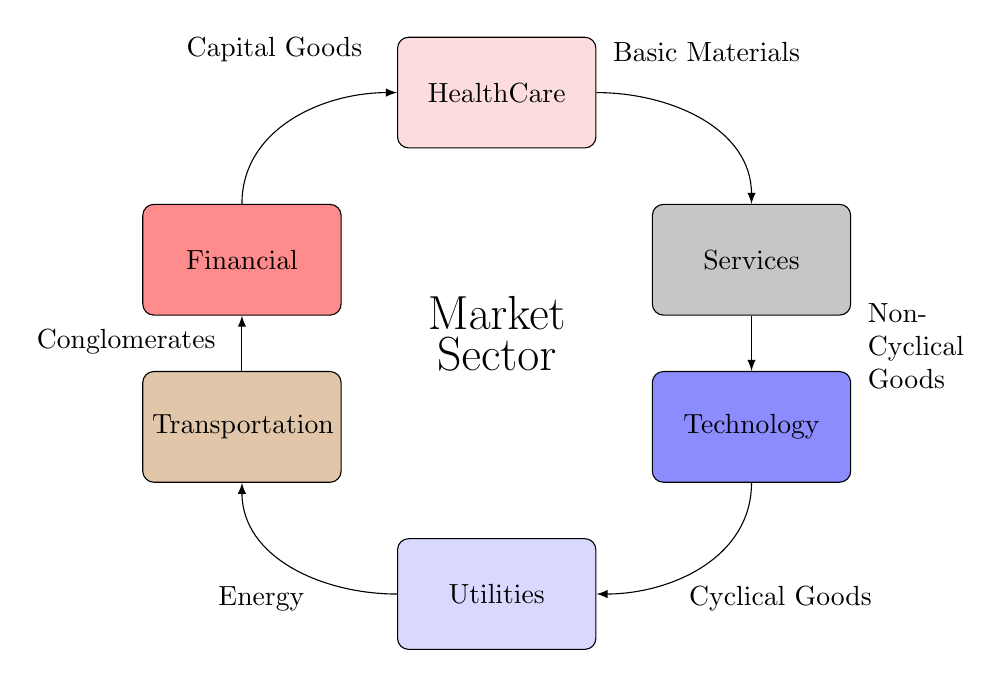
\begin{tikzpicture}[
    node distance=2em and 2em,
    block/.style={rectangle, draw, 
    text width=6.5em, text centered, rounded corners, minimum height=4em},
    line/.style={draw, -latex},
    ]

    \node [block, fill=gray!15!red!15] (hc) {HealthCare};
    \node [block, fill=gray!45, below right= of hc] (serv) {Services};
    \node [block, fill=blue!45, below = of serv] (tech) {Technology};
    \node [block,fill=blue!15, below left= of tech] (util) {Utilities};
    \node [block,fill=brown!45, above left= of util] (trans) {Transportation};
    \node [block, fill=red!45, above = of trans] (fin) {Financial};
    % Connections
    \path [line] (hc.east) to[out=0, in=90] (serv.north);
    \path [line] (serv.south) -- (tech);
    \path [line] (tech.south) to[out=-90, in=0] (util.east);
    \path [line] (util.west) to[out=180, in=-90] (trans.south);
        \path [line] (trans.north) -- (fin);
    \path [line] (fin.north) to[out=90, in=180] (hc.west);
    
    % Market Sectors label
    \node [draw=none, below = 5em of hc, text width = 2cm, align = center] (label) {\LARGE Market \\[1mm] Sector};
    
    \node [above left = -3em and 3em of util] () {Energy};
    \node [above right = -3em and 3em of util] () {Cyclical Goods};
    \node [above right = -1em and 0.25em of tech, text width = 3.5em] () {Non-Cyclical Goods};
    \node [above right = -1.25em and 0.25em of hc, text width = 7em] () {Basic Materials};
    \node [above left = -1.25em and 0.25em of hc, text width = 7em] () {Capital Goods};
    \node [above left = 0.25em and -3em of trans] () {Conglomerates};
\end{tikzpicture}
\end{document}